\documentclass[oneside,openany]{article}

%cerca pacchetto per togliere i rientri dai capitoli
%aggiungi cite dei siti
\usepackage[utf8x]{inputenc}
\usepackage[english]{babel}
\usepackage{enumerate}
\usepackage{graphicx}
\usepackage{multirow}
\usepackage{subfig}
\usepackage{verbatim}
\usepackage{todonotes}


\usepackage{graphicx,subcaption}

\graphicspath{ {./img/} }
\bibliographystyle{unsrt}

\title{Urban Sound Classification}
\author{Alessia Lombarda, Andrea Valota}
\date{Aprile 2022}

\begin{document}

    \begin{titlepage}
	
	    \begin{figure}
	        \centering
	    	
\includegraphics[width=\textwidth]{MINERVA.jpg}
	    	\vspace{0.5 cm}
	    \end{figure}
	

    \begin{center}
    {\Large Corso di Laurea Magistrale in Informatica}
    \end{center}

    \begin{center}
    \vspace{1 cm}
    {\huge \textsc{ Urban Sound Classification } }
    \end{center}
    \begin{center}
    \vspace{1 cm}
    {\LARGE Alessia Lombarda, Andrea Valota}
    \end{center}
    
    \par
        \vspace{1 cm}
    \vfill
    \end{titlepage}
    
    \frontmatter
    
    \tableofcontents
    \vfill
    \textit{We declare that this material, which we now submit for assessment, is entirely our own work and has not been taken from the work of others, save and to the extent that such work has been cited and acknowledged within the text of our work. We understand that plagiarism, collusion, and copying are grave and serious offences in the university and accept the penalties that would be imposed should I engage in plagiarism, collusion or copying. This assignment, or any part of it, has not been previously submitted by us or any other person for assessment on this or any other course of study.}
    \newpage
    \pagestyle{plain}
    \mainmatter
    
    
    \section*{Introduction}
    \addcontentsline{toc}{section}{Introduction}
    The goal of this project is the implementation of neural network models to perform classification of audio samples from \textit{UrbanSound8k dataset}\footnote[1]{\url{https://urbansounddataset.weebly.com/urbansound8K.html}}.\\
    To achieve this goal different types of features, feature selection methods and various types of MLP and CNN architectures have been used.\\
    The dataset is made of sound excerpts from 10 classes drawn from the urban sound taxonomy: air conditioner, car horn, children playing, dog bark, drilling, engine idling, gun shot, jackhammer, siren and street music.\\
    The project has been developed using Python; we used the \textit{Librosa} library to load files and extract features and \textit{TensorFlow 2} to build and train the models.
    All the code and the experimental results can be found in the Github repository \textit{UrbanSoundClassification}\footnote[2]{\url{https://github.com/AlessiaLombarda/UrbanSoundClassification}}.\\
    The report is structured as follows: in Section \ref{section:dataset} the dataset is described and analyzed, in Section \ref{section:features} the feature extraction and feature selection processes are illustrated, focusing on the various feature datasets that will be used to train the models. In Section \ref{section:models} are then explained the MLP and CNN models implemented to perform the classification task, the selected parameters and the obtained results.
    
    \newpage
    \section{UrbanSound8K Dataset}
    \label{section:dataset}
    
    The UrbanSound8K dataset is presented in the paper \textit{A Dataset and Taxonomy for Urban Sound Research}~\cite{salamon2014dataset}. The dataset contains $8732$ labeled sound excerpts ($\leq4$s) of urban sounds from $10$ classes: \textit{air\_conditioner}, \textit{car\_horn}, \textit{children\_playing}, \textit{dog\_bark}, \textit{drilling}, \textit{engine\_idling}, \textit{gun\_shot}, \textit{jackhammer}, \textit{siren}, and \textit{street\_music}. Those classes are drawn from the urban sound taxonomy.\\
    The files are in WAV format; the sampling rate, bit depth, and number of channels are the same as those of the original file uploaded to Freesound (and hence may vary from file to file).\\
    Together with the dataset a metadata file is attached, providing useful information about the audio files; in particular for each file are known:
    
    \begin{itemize}
    \item \textit{slice\_file\_name}: the name of the audio file,
    \item \textit{fsID}: the Freesound ID of the recording from which this excerpt is taken,
    \item \textit{start} and \textit{end}: the start and end time of the slice in the original Freesound recording,
    \item \textit{salience}: a salience rating of the sound ($1$ = foreground, $2$ = background),
    \item \textit{fold}: the fold number ($1$-$10$) to which this file has been allocated,
    \item \textit{classID}: a numeric identifier of the sound class,
    \item \textit{class}: the class name.
    \end{itemize}
    
    The files are pre-sorted into ten folds (folders named \textit{fold1}-\textit{fold10}). As assigned \textit{fold1}, \textit{fold2}, \textit{fold3}, \textit{fold4} and \textit{fold6} are used for training, the remainings for test.
    
    \subsection{Preprocessing}
    \label{subsection:preprocessing}
    In the UrbanSound dataset the different audio files have different sampling frequencies: to better handle data in the training phase, data have been converted (using Librosa tools) so that they all have a final sampling frequency of $44100$ Hz. This frequency was chosen because the majority of the audio files already had that sampling rate, as can be observed in Table~\ref{table:fs}. Furthermore in this phase the channels for all the files is set to \textit{mono} (one channel). 
    The audio files also present different duration; for this reason, they all have been padded with zeros to match the length of the longest file (four seconds).\\
    To better explore the train and test sets, the number of files belonging to each class in the two sets is presented in Table~\ref{table:classes}. 
    The data shows that the number of samples for each class are fairly distributed between the two sets, with the exception of the \textit{Jackhammer} and \textit{Siren} class, and almost all the classes have similar number of total samples, with the \textit{Gun shot} and \textit{Car horn} classes being underrepresented. 

    \begin{table}
    \hspace{-1.5cm}
    \parbox{.45\linewidth}{
\begin{center}
    \begin{tabular}{ |c|c|c| } 
    \hline
    \textbf{Sampling Rate (Hz)} & \textbf{Number of files} \\ 
    \hline
    $\leq$11024 & 19 \\ 
    11025 & 39 \\ 
    16000 & 45 \\ 
    22050 & 44 \\
    24000 & 82 \\ 
    32000 & 4 \\ 
    44100 & 5370 \\
    48000 & 2502 \\ 
    96000 & 610 \\ 
    192000 & 17 \\
    \hline
    \end{tabular}
    \captionsetup{justification=centering}
    \caption{Number of audio files with a given sampling rate}
    \label{table:fs}
    \end{center}
}
\hfill
\hspace{1cm}
\parbox{.45\linewidth}{
\begin{center}
    \begin{tabular}{ |c|c|c|c| } 
    \hline
    \textbf{Class} & \textbf{Train set} & \textbf{Test Set} \\ 
    \hline
    Air conditioner & 500 & 500\\
    Car horn & 208 & 221\\
    Children playing & 500 & 500\\
    Dog bark & 500 & 500\\
    Drilling & 500 & 500\\
    Engine idling & 517 & 483\\
    Gun shot & 190 & 184\\
    Jackhammer & 548 & 452\\
    Siren & 536 & 393\\
    Street music & 500 & 500\\
    \hline
    \end{tabular}
    \captionsetup{justification=centering}
    \caption{Absolute frequency of the classes in train and test set}
    \label{table:classes}
    \end{center}}
\end{table}

    \section{Feature Extraction and Feature Selection}
    \label{section:features}
    
    \subsection{Feature extraction}
    \label{subsection:feature_extraction}
    The preprocessed dataset obtained as illustrated in Section~\ref{subsection:preprocessing} is a collection of WAV files of the same length: differences between the different urban sounds categories can be found by simply observing the shape of the files' sound wave, as can be seen in Figure~\ref{fig:audio}.\\
    %decidi se rimpicciolirla
    \begin{figure}[h]
    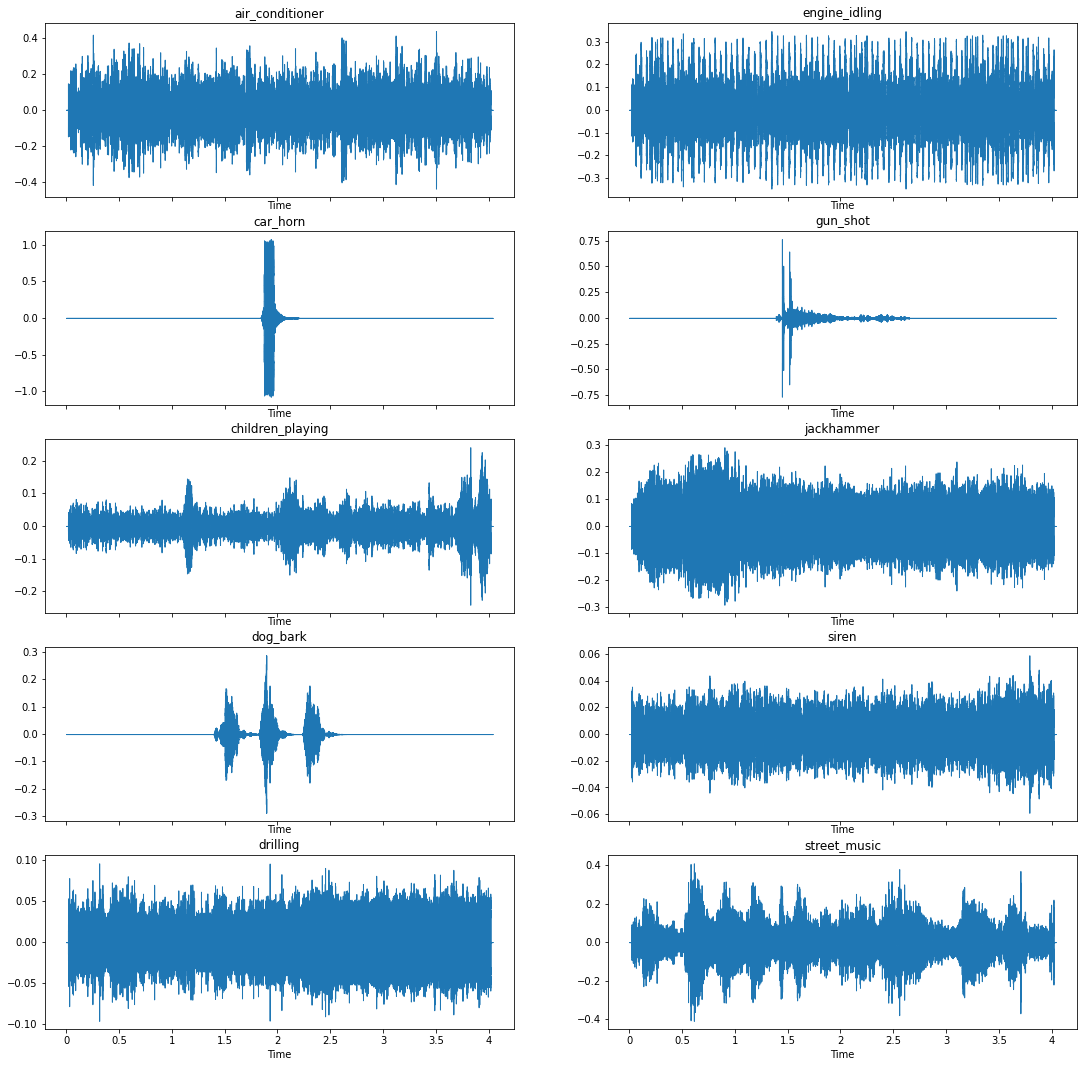
\includegraphics[width=\columnwidth]{audio.png}
    %\centering
    \caption{Audio samples for each category}
    \label{fig:audio}
    \end{figure}
    In order to extract information from the audio files, different features have been selected; the first features extracted are the one returning a single value for each file:
    \begin{itemize}
    \item \textit{min}: the minimum value of amplitude reached by the signal,
    \item \textit{max}: the maximum value of amplitude reached by the signal,
    \item \textit{median}: the median value of amplitude in the audio file,
    \item \textit{mean}: the mean value of amplitude in the audio file,
    \item \textit{var}: the overall variance in the audio file,
    %\item \textit{coeff\_var}: the coefficient of variation,
    \item \textit{rms}: the root mean square of the file, computed as \[RMS=\sqrt{\frac{1}{N}\sum_{k=1}^N x_k^2},\] where $N$ is the length of the audio file and $x_k$ the $k$-th audio sample.
    \end{itemize}
    More complex features have been then selected; these metrics are computed dividing the signal in windows with \textit{window length} set to $2048$ samples and \textit{hop length} of $1024$ (so that all the windows have $50\%$ of overlapping). To summarize the resulting values, five different metrics (minimum, maximum, median, mean and variance) have been chosen. 
    The selected features are:
    \begin{itemize}
    \item \textit{energy}: the root-mean-square value for each window, which can be interpreted as the loudness or energy of the audio file,
    \item \textit{ZCR}: the number of time-domain zero-crossings within a processing window, computed as \[ZCR=\frac{1}{M-1} \sum_{m=0}^{M-1} |sign(x_m)-sign(x_m-1)|,\] where $sign$ is $1$ for positive arguments and $0$ otherwise, $M$ is the total number of samples in a processing window and $x_m$ is the value of the $m$-th sample. 
    This metric is widely used is speech/music classification~\cite{Andersson1030847}. 
    \item \textit{spectral centroid}: a metric indicating the center of gravity of the frequency power spectrum; it is a measure that states if the spectrum contains a majority of high or low frequencies. It is computed as \[SC(t)=\frac{\sum_{k}freq(k)\cdot S(k,t)}{\sum_{j}S(j,t)},\] where $S$ is a magnitude spectrogram, and $freq$ is the array of frequencies of the rows of $S$,
    \item \textit{spectral bandwidth}: the deviation of the spectrum from the spectral centroid; it measures if the power spectrum is concentrated around the centroid or if it is spread out over the spectrum. It is computed as \[ (\sum_{k} S(k, t) \cdot (freq(k, t) - SC(t))^2)^\frac{1}{2},\] 
    \item \textit{spectral rolloff}: metric that defines how high in the frequency spectrum a certain part of the energy ($85\%$) lies,
    \item \textit{spectral flatness}: metric that quantifies how much noise-like a sound is, as opposed to being tone-like. A high spectral flatness (closer to $1.0$) indicates that the spectrum is similar to white noise.
    \end{itemize}
    
    \noindent Furthermore, other two important features have been extracted: the MFCC values and the Chromagram.
    \paragraph{MFCC}
    The \textit{Mel Frequency Cepstral Coefficients} (MFCCs) are a type of cepstral representation of the signal, where the frequency bands are distributed according to the Mel-scale, instead of the linearly spaced approach. The Mel scale is a perceptually motivated scale of frequency intervals, which, if judged by a human listener, are perceived to be equally spaced.\\
    The pipeline to compute MFCCs is described in Figure~\ref{fig:mfcc_pipeline}: the audio signal is divided into frames by applying a window function at fixed intervals.\\ 
    \begin{figure}[h]
    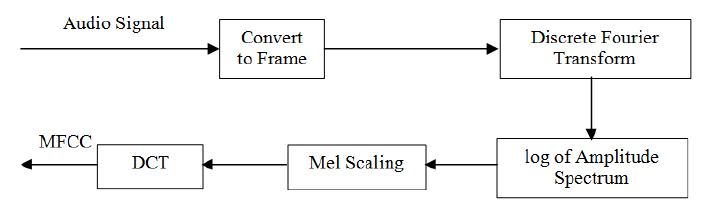
\includegraphics[width=\columnwidth]{mfcc_pipeline.png}
    %\centering
    \caption{Process to create MFCC features}
    \label{fig:mfcc_pipeline}
    \end{figure}
    On each windowed signal the Fourier Transform is applied.
    The obtained powers of the spectrum are then mapped onto the mel scale; the logs of the powers at each of the mel frequencies are taken. Lastly the discrete cosine transform of the list of mel log powers is computed, as if it were a signal: the MFCCs are the amplitudes of the resulting spectrum.\\
    MFCCs are extracted from the UrbanSound8K dataset as described in~\cite{salamon2014dataset}: $40$ Mel bands are computed but only the first $25$ coefficients are kept (the $0$-th coefficient is excluded); the per-frame values for each coefficient are summarized across time using the following summary statistics: minimum, maximum, median, mean, variance, skewness, kurtosis and the mean and variance of the first and second derivative.
    
    \paragraph{Chromagram}
    The \textit{chroma vector} is a $12$-element representation of the spectral energy of the signal; this feature is computed by grouping the DFT coefficients of a short-term window in 12 bins. Each bin represents one of the 12 equal-tempered pitch classes of Western-type music (semitone spacing)~\cite{chroma}.\\
    The matrix representation of the sequence of the chroma vectors is known as \textit{Chromagram}; in this work the chromagram was summarized using minimum, maximum, median, mean and variance, extracted for each bin representing a pitch.
    
    \subsection{Image dataset}
    \label{subsection:img_dataset}
    Some of the features that can be extracted from the audio files can be treated as images; this property can lead to the usage of specific image processing approaches for classification, like \textit{Convolutional Neural Networks}. 
    
    \paragraph{Mel spectrogram} 
    The Mel spectrogram is a Mel-scaled spectrogram: the audio signal is mapped from the time domain to the frequency domain using the Fast Fourier Transform, performed on overlapping windowed segments of the audio signal. The frequency axis is then converted to a log scale and the amplitude to decibels, to obtain the spectrogram.\\ 
    The Mel Spectrogram is computed on the UrbanSound8K dataset using a \textit{window length} of $2048$ and \textit{hop length} of $1024$. The resulting matrix can be seen as an image, as shown in Figure~\ref{fig:mel}.

    \paragraph{MFCC}
    The MFCCs are computed as explained above. The MFCCs can be seen as a 2D image: for each file the image will have as many rows as the number of considered coefficients and as many columns as the number of windows extracted from the audio file. An example of the resulting image is shown in Figure~\ref{fig:mfcc}.
    
    \paragraph{Chromagram}
    The Chromagram is computed as explained above. The Chromagram itself is a matrix and can be seen as an image with one row for each pitch class and one column for each window extracted from the audio file. The possible resulting image is shown in Figure~\ref{fig:chroma}.

    \begin{figure}[!h]
        \hspace{-2cm}
	    %\centering
	    \subfloat[\hspace{0.3cm}\emph{Sample image of Mel Spectrogram}]
	    {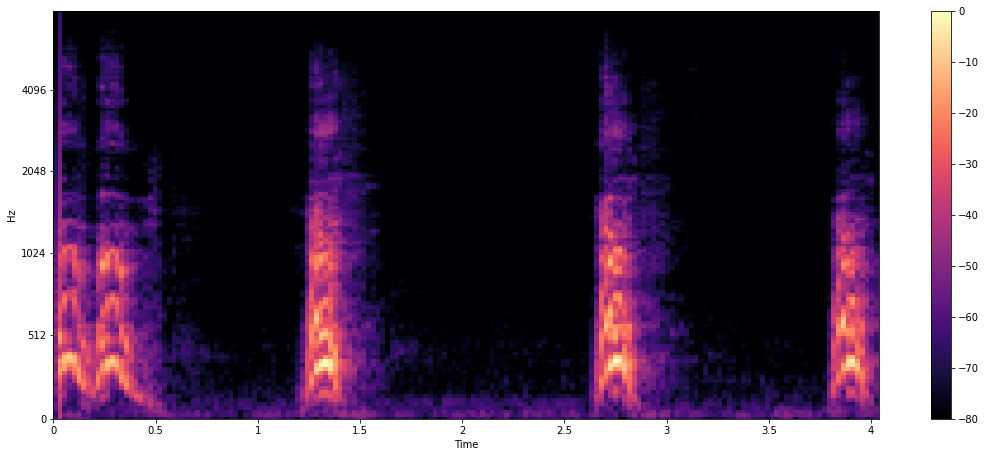
\includegraphics[width=8cm,height=5cm]{mel.png}\label{fig:mel}} \quad
	    \subfloat[\hspace{0.3cm}\emph{Sample image of MFCC}]
	    {\hspace{0.4cm}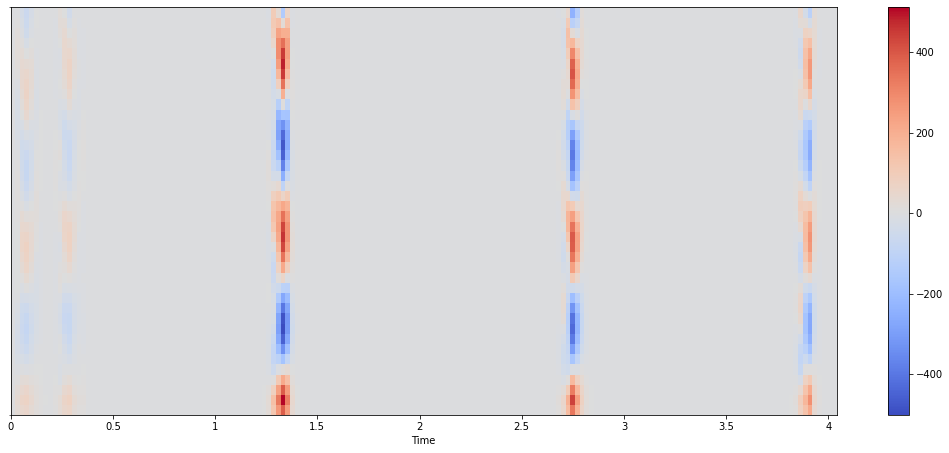
\includegraphics[width=8cm,height=5cm]{mfcc.png}\label{fig:mfcc}} \quad \\
	    \subfloat[\hspace{1.5cm}\emph{Sample image of Chromagram}]
	    {\hspace{2cm}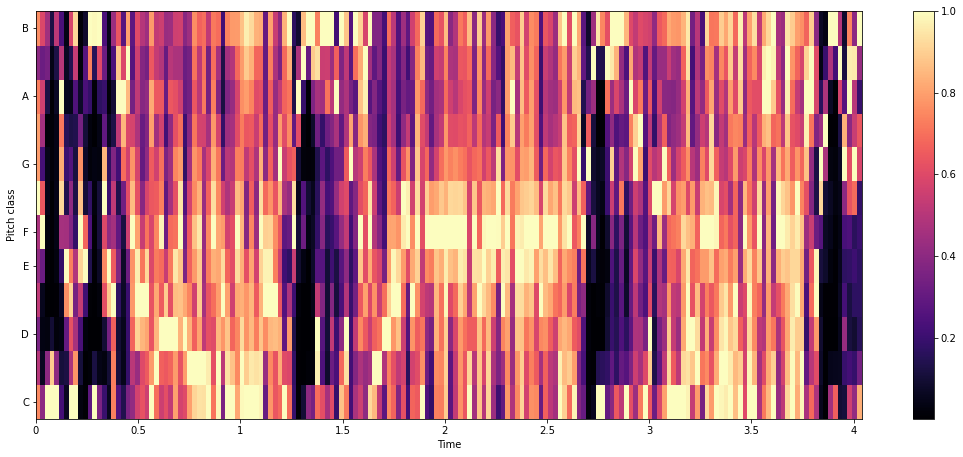
\includegraphics[width=8cm,height=5cm]{chroma.png}\label{fig:chroma}} 
	\end{figure}
    
    \subsection{Feature selection}
    \label{subsection:feature_selection}
    Different subsets of the features explained in Sections~\ref{subsection:feature_extraction} and \ref{subsection:img_dataset} have been used to train different models: mainly the first subset consisted in a set of the basic features, containing the basic statistics over the raw data and the more advanced ones like energy, ZCR and metrics on the spectrum of the signal; a broader set of features used to train other models also contains MFCCs and chroma features.\\
    Another approach followed is the PCA technique to perform feature selection: the \textit{Principal Component Ananlysis} is the process of computing the principal components and using them to perform a change of basis on the data, sometimes using only the first few principal components and ignoring the rest. The PCA is commonly used for dimensionality reduction by projecting each data point onto the first few principal components to obtain lower-dimensional data, while preserving as much of the data's variation as possible. The first principal component can equivalently be defined as a direction that maximizes the variance of the projected data~\cite{pca}.\\ 
    In the considered dataset, the PCA was applied to the whole feature dataset, experimenting different variance thresholds.
    
    \section{Proposed models and experiments}
    \label{section:models}
    In this section the different models implemented to perform the classification task are illustrated. Each model was implemented using \textit{keras}\footnote{https://www.tensorflow.org/api_docs/python/tf/keras} library; the tools used to run the code are \textit{Colab} notebooks using a GPU runtime.\\
    For each model multiple experiments have been performed, evaluating the performances of the models varying the \textit{number of epochs} and the \textit{batch size}; for each combination of these hyperparameters $3$ experiments have been executed, in order to obtain an average goodness of the model and its standard deviation. The metric used to evaluate the model performance is the \textit{accuracy}, that computes how often predictions made by the model are equal to the data labels. A confusion matrix has also been computed in order to better analyze how the prediction errors are distributed.
    For simplicity, in the tables proposed in the next sections results will be averaged on the three experiments.\\
    Each model is trained over a train set containing data from \textit{fold1}, \textit{fold2}, \textit{fold3}, \textit{fold4}, \textit{fold6} and tested on each of the remaining folds independently; the accuracy and its standard deviation on each fold will also show differences in how the composition of the folds influences the goodness of the classification.
    
    \subsection{Raw data model}
    \label{subsection:raw_model}
    The first architecture proposed to perform classification over audio files dataset directly works on raw data (already preprocessed as described in Section~\ref{subsection:preprocessing}). The training phase of the model on the obtained raw data resulted to be very time and resources consuming, running out of available Colab resources. To avoid it, data have been preprocessed again from the original dataset lowering the sampling frequency to $22050$ Hz, so that the dimension of each raw file halved.\\
    Since there are no feature extracted from these data, the considered model is a 1D-CNN with a final dense layer; the activation function chosen for each layer is the \textit{ReLu} (Rectifying Linear Unit, used in the CNNs to mitigate the problem of vanishing gradient) except for the last layer, that uses a \textit{Softmax} activation function. The Softmax is used to make the final output a vector in which each element represents the probability for a data point to belong to one of the ten possible urban sound categories.\\
    Pooling and Dropout are also introduced to improve the performances of the network: \textit{MaxPooling} is used after each convolution step and the predefined \textit{pool size} is set to $2$ while \textit{Dropout} is applied after the pooling, and its \textit{rate} is set to $0.2$ (increasing the dropout probability led to worse performances by the models).\\
    Before the final Dense layer, a \textit{Global Average Pooling} is performed to flatten data.\\
    Among the possible configurations of number of layers, filter dimension and padding, the following model had the best performance on our data.
    %compatta
    \begin{itemize}
    \item \textbf{Layer 1}:
    \begin{itemize}
        \item A \textit{1D convolutional layer} of $64$ filters with kernel size $5$,
        \item A \textit{Max Pooling layer},
        \item A \textit{Dropout layer}.
    \end{itemize}
    
    \item \textbf{Layer 2}:
    \begin{itemize}
        \item A \textit{1D convolutional layer} of $128$ filters with kernel size $4$,
        \item A \textit{Max Pooling layer},
        \item A \textit{Dropout layer}.
    \end{itemize}
    \item \textbf{Layer 3}:
    \begin{itemize}
        \item A 1D convolutional layer of $256$ filters with kernel size $3$,
        \item A Max Pooling layer,
        \item A Dropout layer.
    \end{itemize}
    \item \textbf{Layer 4}:
    \begin{itemize}
        \item A \textit{1D convolutional layer} of $512$ filters with kernel size $2$,
        \item A \textit{Max Pooling layer},
        \item A \textit{Dropout layer}.
    \end{itemize}
    \item \textbf{Global Average Pooling}
    \item \textbf{Layer 5:}
    \begin{itemize}
        \item A \textit{Dense layer} of size $10$
    \end{itemize}
    \end{itemize}
    The obtained model has some layers with lots of filters: this results in a high number of trainable parameters. Reducing the number of parameters led the model to underfit; furthermore, the architecture defined above is very hard to train in terms of computational time and resources: for this reason, only few experiments have been executed on it. Generally speaking, increasing the number of epochs improve both train and test accuracy, suggesting that a longer training should be done; unfortunately that cannot be experimented due to the previously illustrated limitations.\\
    Experiments have been performed with a variable number of epochs and batch size; the selected values for the batch size are $16$ and $32$ since a larger batch size made Colab stop the execution due to limitations in the memory usage. The values chosen for the number of epochs are $50$, $70$ and $100$.
    Setting a batch size of $16$, the overall accuracy of the model lies between $40\%$ and $48\%$, increasing as the number of epochs grows; the same happens with a batch size of $32$, in which the accuracy slightly increases up to $50\%$.
    
    \subsection{Base statistics model}
    \label{subsection:base_model}
    The base model is built over a feature dataset composed of the basic features illustrated in the first part of Section~\ref{subsection:feature_extraction}, that are basic statistics over data, energy, ZCR and statistics over the spectrum; since there already are features extracted from the data, the proposed model is a Multi-Layer Perceptron. \\
    Before feeding the network with the features, a normalization step was performed; this preprocessing phase is needed because results obtained by the same model on non-scaled features were close to random-like behaviour.\\
    The MLP is composed of dense fully-connected layers; for each layer but the last, the \textit{ReLu} function is set as activation function while, for the last layer, the selected function is a \textit{Softmax}, to perform the final classification. Among the examined architectures, the one performing best on the considered data is the following:
    
    \begin{itemize}
    \item \textbf{Layer 1}: a \textit{Dense layer} of size $1024$,
    \item \textbf{Layer 2}: a \textit{Dense layer} of size $512$.
    \item \textbf{Layer 3}: a \textit{Dense output layer} of size $10$.
    \end{itemize}
    The MLP is composed by only two hidden layers: experiments have shown that the MLP with few large layers outperform architectures with many short ones.
    The average results of the experiments performed using the described model are shown in Table~\ref{table:base}.
    \begin{table}[ht]
        %\hspace{-0.7cm}
        \resizebox{\columnwidth}{!}{
        \begin{tabular}{|c|c|c|c|c|}
        \hline
        \textbf{Batch size} & \textbf{Epochs} & \textbf{Train accuracy} & \textbf{Test accuracy} & \textbf{Test accuracy std} \\
        \hline
        \multirow{4}{4em}{\centering \textbf{32}}  & 30 & 80.91\% & 48.45\% & 1.84\\
        & 40 & 85.59\% & 48.37\% & 2.40\\
        & 50 & 88.17\% & 48.27\% & 2.28\\
        & 70 & 92.16\% & 46.28\% & 2.81\\
        \hline
        \multirow{4}{4em}{\centering \textbf{64}}  & 30 & 76.43\% & 49.27\% & 3.09\\
        & 40 & 81.12\% & 49.26\% & 2.93\\
        & 50 & 84.20\% & 48.43\% & 3.25\\
        & 70 & 88.93\% & 48.64\% & 2.42\\
        \hline
        \multirow{4}{4em}{\centering \textbf{128}}  & 30 & 71.66\% & 47.59\% & 2.62\\
        & 40 & 76.20\% & 47.89\% & 3.02\\
        & 50 & 79.32\% & 50.12\% & 2.93\\
        & 70 & 83.39\% & 49.62\% & 3.22\\
        \hline
        \end{tabular}
        }
        \caption{Results obtained by the MLP trained on the Base statistics dataset}
        \label{table:base}
    \end{table}
    
    \subsection{Advanced statistics model}
    \label{subsection:adv_model}
    Advanced feature dataset includes all features already mentioned in Section~\ref{subsection:base_model}, together with MFCCs and chroma vectors. In this case features have been rescaled too; experiments performed on non-rescaled features led to accuracies close to the one of a random classifier. \\
    For advanced feature dataset two different models are proposed: \textit{Advanced Model 1} is the MLP already illustrated in Section~\ref{subsection:base_model} while \textit{Advanced Model 2} is another MLP with a higher number of smaller layers. As in the previous model, the activation function used for all layers but the last is the \textit{ReLu}; the last layer uses \textit{Softmax} instead. The model structure is defined as follows:
    \begin{itemize}
    \item \textbf{Layer 1}: a \textit{Dense layer} of size $64$
    \item \textbf{Layer 2}: a \textit{Dense layer} of size $64$
    \item \textbf{Layer 3}: a \textit{Dense layer} of size $32$
    \item \textbf{Layer 4}: a \textit{Dense layer} of size $16$
    \item \textbf{Layer 5}: a \textit{Dense output layer} of size $10$
    \end{itemize}
    
    The results obtained on both models are shown in Table~\ref{table:adv}.
    \\
    \begin{table}[ht]
        \hspace{0cm}
        \resizebox{\columnwidth}{!}{
        \begin{tabular}{|c|c|c|c|c|}
        \hline
        \multicolumn{5}{|c|}{\textbf{Advanced model 1}}\\
        \hline
        \textbf{Batch size} & \textbf{Epochs} & \textbf{Train accuracy} & \textbf{Test accuracy} & \textbf{Test accuracy std} \\
        \hline
        \multirow{4}{4em}{\centering \textbf{32}}  & 40 & 87.55\% & 53.24\% & 1.64\\
        & 50 & 90.42\% & 53.64\% & 2.03\\
        & 70 & 93.58\% & 52.52\% & 2.08\\
        & 100 & 95.96\% & 52.66\% & 2.73\\
        \hline
        \multirow{4}{4em}{\centering \textbf{64}}  & 40 & 85.99\% & 54.76\% & 2.15\\
        & 50 & 88.92\% & 53.99\% & 2.76\\
        & 70 & 92.66\% & 55.51\% & 1.97\\
        & 100 & 95.07\% & 54.79\% & 1.58\\
        \hline
        \multirow{4}{4em}{\centering \textbf{128}}  & 40 & 83.71\% & 55.41\% & 3.05\\
        & 50 & 86.04\% & 55.71\% & 1.80\\
        & 70 & 89.83\% & 55.22\% & 2.07\\
        & 100 & 94.29\% & 55.55\% & 2.16\\
        \hline
        \multicolumn{5}{|c|}{\textbf{Advanced model 2}}\\
        \hline
        \textbf{Batch size} & \textbf{Epochs} & \textbf{Train accuracy} & \textbf{Test accuracy} & \textbf{Test accuracy std} \\
        \hline
        \multirow{4}{4em}{\centering \textbf{32}}  & 40 & 76.41\% & 52.40\% & 3.39\\
        & 50 & 80.38\% & 53.83\% & 2.19\\
        & 70 & 82.49\% & 53.08\% & 1.80\\
        & 100 & 86.83\% & 53.47\% & 2.37\\
        \hline
        \multirow{4}{4em}{\centering \textbf{64}}  & 40 & 73.36\% & 51.73\% & 2.66\\
        & 50 & 76.66\% & 51.91\% & 3.22\\
        & 70 & 80.59\% & 53.54\% & 1.97\\
        & 100 & 83.77\% & 53.36\% & 2.01\\
        \hline
        \multirow{4}{4em}{\centering \textbf{128}}  & 40 & 69.67\% & 50.36\% & 2.43\\
        & 50 & 71.66\% & 52.71\% & 2.62\\
        & 70 & 76.57\% & 53.95\% & 2.64\\
        & 100 & 81.06\% & 53.37\% & 2.32\\
        \hline
        \end{tabular}
        }
        \caption{Results obtained by the models trained on the Advanced statistic dataset}
        \label{table:adv}
    \end{table}
    \subsection{MLP model on PCA features}
    \label{subsection:pca_model}
    The PCA technique is described in Section~\ref{subsection:feature_selection}; the PCA was applied to the whole feature dataset.
    Experiments on the PCA dataset have been performed selecting values for the \textit{variance threshold} of $90\%$, $95\%$, $98\%$ and $99\%$. \\
    The considered architecture is a MLP; the activation functions are chosen as before. The network is defined as follows:
    \begin{itemize}
    \item \textbf{Layer 1}: a \textit{Dense layer} of size $64$,
    \item \textbf{Layer 2}: a \textit{Dense layer} of size $32$,
    \item \textbf{Layer 3}: a \textit{Dense layer} of size $10$.
    \end{itemize}
    The network is composed by two layers: experiments on different architectures have shown that increasing the number of layers leads to a worse overall accuracy. Furthermore, increasing or decreasing the layers' dimension doesn't seem to affect the test accuracy while a variation in the train accuracy is observed (this holds if the dimension of the layers is kept in a reasonable range of values, otherwise we incur in overfitting or underfitting).\\
    The results of the experiments performed on this architecture are summarized in Table~\ref{table:pca}. As can be seen, setting a variance threshold of $98\%$ leads to an overall accuracy slightly better than the one obtained with lower variance thresholds.
    
    \begin{table}[!ht]
    %\hspace{-2.1cm}
    \resizebox{\columnwidth}{!}{
    \begin{tabular}{|c|c|c|c|c|c|}
    \hline
        \textbf{PCA Variance} & \textbf{Batch Size} & \textbf{Epochs} & \textbf{Train accuracy} & \textbf{Test accuracy} & \textbf{Test accuracy std} \\ 
        \hline
        \multirow{9}{4em}{\centering \textbf{0.9}} & \multirow{3}{4em}{\centering \textbf{32}} & 20 & 79.28\% & 53.38\% & 2.74 \\ 
        & & 30 & 83.46\% & 55.30\% & 2.71 \\ 
        & & 50 & 88.35\% & 53.13\% & 1.46 \\ 
        \cline{2-6}
        & \multirow{3}{4em}{\centering \textbf{64}} & 20 & 76.67\% & 54.52\% & 2.33 \\ 
        & & 30 & 80.75\% & 53.19\% & 2.43 \\ 
        & & 50 & 86.11\% & 54.31\% & 1.98 \\ 
        \cline{2-6}
        & \multirow{3}{4em}{\centering \textbf{128}} & 20 & 73.16\% & 53.30\% & 2.38 \\
        & & 30 & 76.92\% & 53.26\% & 1.95 \\ 
        & & 50 & 82.00\% & 53.72\% & 1.83 \\ 
        \hline
        \multirow{9}{4em}{\centering \textbf{0.95}} & \multirow{3}{4em}{\centering \textbf{32}} & 20 & 83.84\% & 55.71\% & 1.60 \\ 
        & & 30 & 88.31\% & 54.89\% & 1.70 \\ 
        & & 50 & 93.75\% & 53.66\% & 1.59 \\ 
        \cline{2-6}
        & \multirow{3}{4em}{\centering \textbf{64}} & 20 & 80.45\% & 54.54\% & 2.21 \\ 
        & & 30 & 85.17\% & 55.21\% & 2.24 \\
        & & 50 & 90.63\% & 54.99\% & 1.51 \\ 
        \cline{2-6}
        & \multirow{3}{4em}{\centering \textbf{128}} & 20 & 76.86\% & 55.04\% & 1.89 \\ 
        & & 30 & 80.99\% & 54.79\% & 2.34 \\
        & & 50 & 86.49\% & 55.23\% & 1.97 \\
        \hline
        \multirow{9}{4em}{\centering \textbf{0.98}} & \multirow{3}{4em}{\centering \textbf{32}} & 20 & 88.00\% & 55.44\% & 2.15 \\
        & & 30 & 92.69\% & 55.19\% & 1.42 \\ 
        & & 50 & 97.29\% & 55.39\% & 1.50 \\ 
        \cline{2-6}
        & \multirow{3}{4em}{\centering \textbf{64}} & 20 & 84.44\% & 55.88\% & 2.12 \\ 
        & & 30 & 89.43\% & 56.10\% & 1.78 \\ 
        & & 50 & 94.87\% & 55.96\% & 1.96 \\ 
        \cline{2-6}
        & \multirow{3}{4em}{\centering \textbf{128}} & 20 & 80.02\% & 56.10\% & 1.71 \\ 
        & & 30 & 84.79\% & 55.67\% & 2.48 \\ 
        & & 50 & 90.64\% & 55.66\% & 2.82 \\ 
        \hline
        \multirow{9}{4em}{\centering \textbf{0.99}} & \multirow{3}{4em}{\centering \textbf{32}} & 20 & 88.90\% & 56.16\% & 2.44 \\ 
        & & 30 & 94.01\% & 55.58\% & 1.68 \\ 
        & & 50 & 98.15\% & 55.28\% & 2.61 \\ 
        \cline{2-6}
        & \multirow{3}{4em}{\centering \textbf{64}} & 20 & 85.72\% & 56.26\% & 1.69 \\ 
        & & 30 & 90.43\% & 56.12\% & 2.27 \\ 
        & & 50 & 95.77\% & 55.43\% & 1.77 \\ 
        \cline{2-6}
        & \multirow{3}{4em}{\centering \textbf{128}} & 20 & 81.22\% & 55.64\% & 1.41\\ 
        & & 30 & 85.88\% & 56.13\% & 2.38 \\ 
        & & 50 & 92.10\% & 56.13\% & 2.09 \\ 
        \hline
    \end{tabular}
    }
    \caption{Results obtained by the models trained on the PCA dataset}
    \label{table:pca}
    \end{table}
    
    \subsection{CNN model using Mel spectrogram}
    \label{subsection:mel_model}
    A specific architecture has been developed to work on the Mel spectrogram extracted from the audio files as illustrated in Section~\ref{subsection:feature_extraction}. The network is a 2D-CNN, since the Mel spectrogram can be seen as an image from which features characterizing the different audio sounds categories are extracted.\\
    The network structure is very similar to the one used in Section~\ref{subsection:raw_model} for the \textit{raw model}: it presents the same number of layers and activation function and the same application of pooling and dropout; the only difference is that in this case a 2D convolution is performed and the layers have respectively dimension $16$, $32$, $64$, $128$ while the kernels are $5$x$5$, $4$x$4$, $2$x$2$ and $2$x$2$.
    The results obtained by this model are summarized in Table~\ref{table:mel}.
    
    \begin{table}[!ht]
    %\hspace{-0.7cm}
    \resizebox{\columnwidth}{!}{
    \begin{tabular}{|c|c|c|c|c|}
    \hline
        \textbf{Batch size} & \textbf{Epochs} & \textbf{Train accuracy} & \textbf{Test accuracy} & \textbf{Test accuracy std} \\ 
        \hline
        \multirow{4}{4em}{\centering \textbf{32}} & 30 & 75.45\% & 60.54\% & 3.52 \\
        & 40 & 81.49\% & 65.34\% & 4.18 \\ 
        & 50 & 84.46\% & 66.59\% & 3.46 \\ 
        & 70 & 88.04\% & 67.18\% & 4.91 \\ 
        \hline
        \multirow{4}{4em}{\centering \textbf{64}} & 30 & 69.40\% & 56.81\% & 6.62 \\ 
        & 40 & 76.45\% & 62.77\% & 5.13 \\ 
        & 50 & 79.27\% & 60.69\% & 3.95 \\ 
        & 70 & 85.75\% & 67.17\% & 3.58 \\ 
        \hline
        \multirow{4}{4em}{\centering \textbf{128}} & 30 & 63.47\% & 54.67\% & 6.08 \\ 
        & 40 & 68.50\% & 58.77\% & 3.87 \\ 
        & 50 & 71.43\% & 58.63\% & 4.29 \\ 
        & 70 & 78.08\% & 63.85\% & 4.69 \\ 
        \hline
    \end{tabular}
    }
    \caption{Results obtained by the CNN trained on Mel spectrogram}
    \label{table:mel}
    \end{table}
    
    \subsection{CNN model using MFCCs}
    \label{subsection:mfcc_model}
    The network architecture implemented to work on MFCC dataset is the same as the one used on Mel spectrogram, described in Section~\ref{subsection:mel_model}. 
    Using the architecture illustrated above, experiments have been performed: the obtained results are shown in Table~\ref{table:mfcc}. \\
    For this specific feature dataset and network architectures, further experiments have been conduced introducing the \textit{early stopping}. The process of early stopping introduce the validation set and it's used to stop the model before overfitting occurs: using this technique the training of the model interrupts when a given metric (in our case the \textit{validation accuracy}) start decreasing while the train accuracy keep increasing (overfitting).\\
    The training process is repeated $n$ times (being $n$ the number of folds): at each time the validation set is represented by one of the folds and the training set is made of the remaining 4 folds. \\
    Experiments made using this techniques highlighted very short training phases lasting only few epochs, leading to models with low train accuracies (around $70\%$) and consequent low test accuracies. This issue can be explained by the fact that using one fifth of the training set as validation further reduce the train set size to the $40$\% of the total amount of data: for this reason underfitting incurs.
    According to this hypotesis the early stopping technique was not used in all the proposed experiments, since it leads to worse performances of the model.
    
    \begin{table}[ht]
        %\hspace{-0.7cm}
        \resizebox{\columnwidth}{!}{
        \begin{tabular}{|c|c|c|c|c|}
        \hline
        \textbf{Batch size} & \textbf{Epochs} & \textbf{Train accuracy} & \textbf{Test accuracy} & \textbf{Test accuracy std} \\
        \hline
        \multirow{4}{4em}{\centering \textbf{32}}  & 30 & 97.94\% & 55.72\% & 2.75\\
        & 40 & 98.30\% & 54.71\% & 3.34\\
        & 50 & 98.46\% & 54.81\% & 2.00\\
        & 70 & 99.45\% & 53.88\% & 3.39\\
        \hline
        \multirow{4}{4em}{\centering \textbf{64}}  & 30 & 97.08\% & 54.80\% & 2.07\\
        & 40 & 98.60\% & 56.32\% & 3.24\\
        & 50 & 99.33\% & 55.29\% & 2.87\\
        & 70 & 98.76\% & 54.74\% & 2.98\\
        \hline
        \multirow{4}{4em}{\centering \textbf{128}}  & 30 & 93.39\% & 54.02\% & 2.35\\
        & 40 & 96.51\% & 55.23\% & 1.79\\
        & 50 & 97.24\% & 55.01\% & 3.50\\
        & 70 & 99.03\% & 56.47\% & 2.06\\
        \hline
        \end{tabular}
        }
        \caption{Results obtained by the CNN trained on MFCC}
        \label{table:mfcc}
    \end{table}
    
    \subsection{CNN model using Chromagram}
    \label{subsection:chroma_model}
    The CNN is the network structure selected to work on chromagram too: in this case, since the input size is quite small (the chromagram is extracted as explained in Section~\ref{subsection:feature_extraction}), the implemented architecture only has 2 hidden layers.
    The model that resulted to be the best performing is the following:
    \begin{itemize}
    \item \textbf{Layer 1}:
    \begin{itemize}
        \item A \textit{2D convolutional layer} of $128$ filters with kernel size $2$x$2$,
        \item A \textit{Max Pooling layer},
        \item A \textit{Dropout layer}.
    \end{itemize}
    \item \textbf{Layer 2}:
    \begin{itemize}
        \item A \textit{2D convolutional layer} of $256$ filters with kernel size $2$x$2$,
        \item A \textit{Max Pooling layer},
        \item A \textit{Dropout layer}.
    \end{itemize}
    \item \textbf{Global Average Pooling}
    \item \textbf{Layer 3:}
    \begin{itemize}
        \item A \textit{Dense layer} of size $10$.
    \end{itemize}
    \end{itemize}
    The results obtained by this model are illustrated in Table~\ref{table:chroma}.
    As can be observed, the best accuracy obtained is around $53\%$; experiments have shown that adding another layer to the network increased the average overall accuracy to around $57\%$. Unfortunately, since the input size is small, the last added layer can't contain the pooling step (this leads to a zero output size of the feature map). In order to keep the structure of the model coherent and meaningful, the model on which experiments have been performed is the one with two layers; another issue supporting this choice is the fact that other architectures seem to outperform this model.
    
    \begin{table}[!ht]
    %\hspace{-0.7cm}
    \resizebox{\columnwidth}{!}{
    \begin{tabular}{|c|c|c|c|c|}
    \hline
        \textbf{Batch size} & \textbf{Epochs} & \textbf{Train accuracy} & \textbf{Test accuracy} & \textbf{Test accuracy std} \\ \hline
        \multirow{4}{4em}{\centering \textbf{32}} & 30 & 58.39\% & 49.54\% & 2.33 \\ \
        & 40 & 61.32\% & 51.91\% & 1.91 \\ 
        & 50 & 62.90\% & 52.74\% & 2.56 \\ 
        & 70 & 66.26\% & 54.07\% & 2.72 \\ 
        \hline
        \multirow{4}{4em}{\centering \textbf{64}} & 30 & 54.32\% & 46.45\% & 2.67 \\ 
        & 40 & 57.66\% & 47.85\% & 2.39 \\ 
        & 50 & 59.74\% & 49.53\% & 2.46 \\ 
        & 70 & 62.86\% & 51.96\% & 2.59 \\ 
        \hline
        \multirow{4}{4em}{\centering \textbf{128}} & 30 & 49.35\% & 42.88\% & 2.99 \\ 
        & 40 & 51.79\% & 44.15\% & 2.61 \\ 
        & 50 & 54.79\% & 45.68\% & 2.34 \\ 
        & 70 & 58.73\% & 49.36\% & 2.18 \\ 
        \hline
    \end{tabular}
    }
    \caption{Results obtained by the CNN trained on Chromagram}
    \label{table:chroma}
    \end{table}
    
    \subsection{Results analysis}
    \label{subsection:results}
    In the previous subsections results obtained by the different architectures are illustrated; in Table~\ref{table:results} the best accuracies obtained for each model are summarized.\\
        \begin{table}[!ht]
    %\hspace{0.2cm}
    \resizebox{\columnwidth}{!}{
    \begin{tabular}{|c|c|c|}
    \hline
        \textbf{Model}  & \textbf{Test accuracy} & \textbf{Test accuracy std} \\ 
        \hline
        \textbf{Raw Model} & \sim50\% & --- \\ \
        \textbf{Base Statistics Model} & 50.12\% & 2.93  \\ 
        \textbf{Advanced Statistics Model} & 55.55\% & 2.16 \\ 
        \textbf{PCA Model} & 56.26\% & 1.69  \\ 
        \textbf{Mel spectrogram Model} & 67.18\% & 4.91\\
        \textbf{MFCC Model} & 56.46\% & 2.06 \\
        \textbf{Chromagram Model} & 54.07\% & 2.72\\
        \hline
    \end{tabular}
    }
    \caption{Best results obtained by the different models}
    \label{table:results}
    \end{table}
    Data shows that the best performances are obtained by the 2D-CNN trained on Mel Spectrogram data, while the worst performing model is the 1D-CNN on raw data (probably due to our computational limits). Observing the standard deviation of the accuracy obtained by the Mel Spectrogram model it can be noticed that, since the value is the highest among all the models, the performance of that CNN varies significantly on each test fold. \\
    Furthermore, as expected the Advanced Statistics model outperforms the Base Statistic one (that is fed with a subset of the features used to train the advanced model); moreover, the PCA model performs better than the Advanced Statistics model and this is expected too since the PCA applied on the advanced feature set retrieves features that are more relevant and better exploit the variance in the data. \\
    The lower accuracy of the Chromagram model is explained by the properties of the data; since the chromagram focuses on finding pitch class profiles that are more relevant in music or similar context, it not useful to discriminate between different kinds of urban noise which represents most of the categories that constitute the dataset.  

    \paragraph{Confusion matrices and classification problems}
    For each model a confusion matrix have been created in order to better understand how the classification errors are distributed. The confusion matrix shows on the diagonal the number of samples correctly classified while the other elements represent the number of samples incorrectly classified.\\
    A general analysis on the models' matrices shows that most of the models tend to misclassify between the \textit{jackhammer} and \textit{drilling} classes and between the \textit{air conditioner} and \textit{engine idling} classes: this is the main reason for which certain models still have relatively low accuracy when the classification on all other classes is way more precise.\\
    Furthermore, as expected the Chromagram model tends to have a better accuracy on the classification of \textit{street music} audio files, that in other models are mixed up with \textit{siren} or \textit{children play} files.
    
    \newpage
    
    \begin{figure}[!ht]
        \hspace{-1.5cm}
	    %\centering
	    \subfloat[\emph{Confusion matrix of Base Model}]
	    {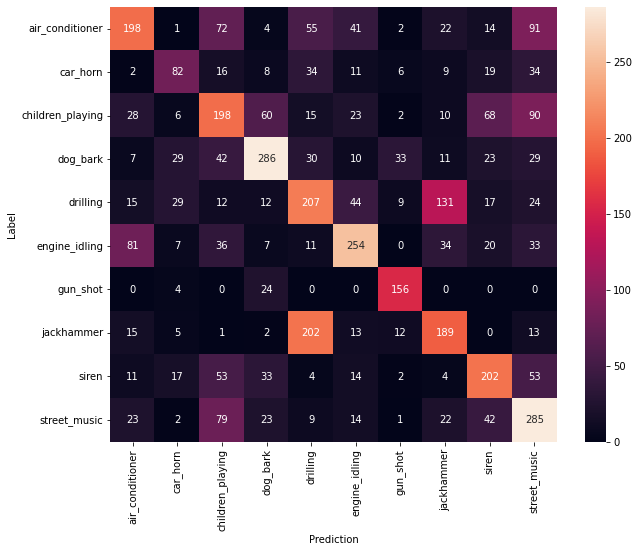
\includegraphics[width=7cm,height=7cm]{mc_base.png}} \quad
	    \subfloat[\emph{Confusion matrix of Chromagram Model}]
	    {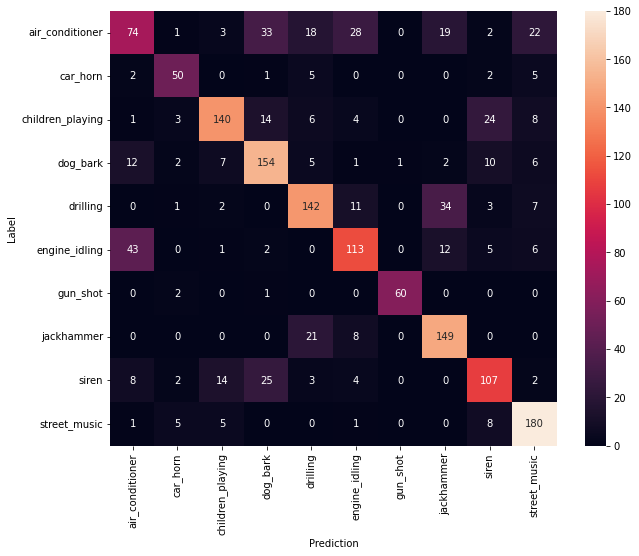
\includegraphics[width=7cm,height=7cm]{mc_chroma.png}} \quad
	    \subfloat[\emph{Confusion matrix of Mel Spectrogram Model}]
	    {\hspace{-1.5cm}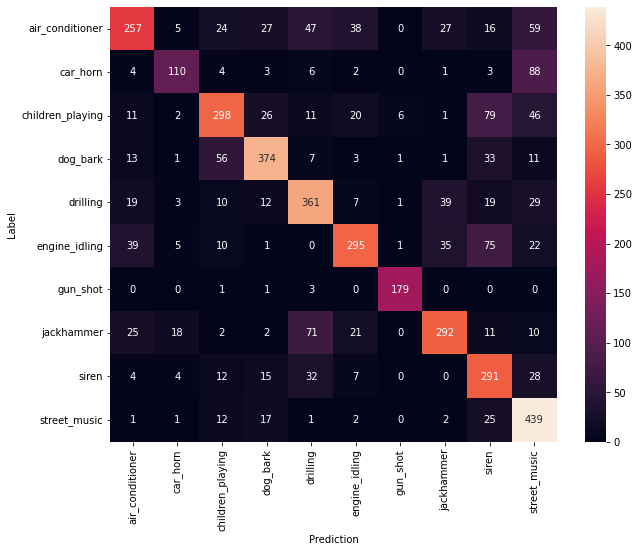
\includegraphics[width=7cm,height=7cm]{mc_mel.png}} \quad
	    \subfloat[\emph{Confusion matrix of Raw Model}]
	    {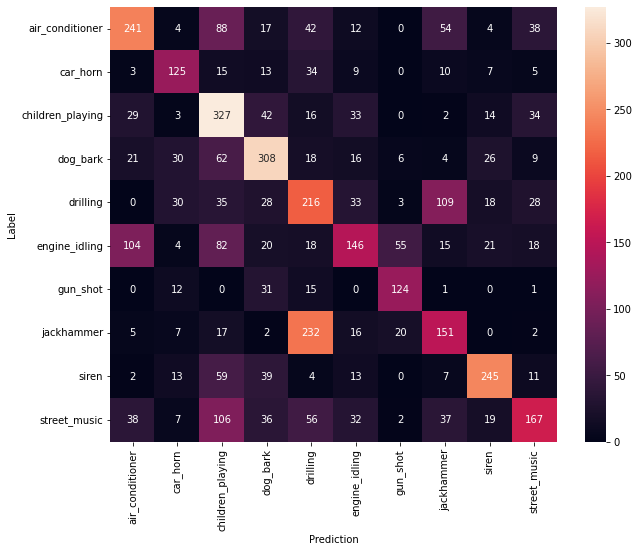
\includegraphics[width=7cm,height=7cm]{mc_raw.png}} \quad
	    \caption{Examples of confusion matrices of some of the models}
	    \label{fig:mc}
	\end{figure}
	
	\newpage

    \section*{Conclusion}
    \addcontentsline{toc}{section}{Conclusions}
    In this report different techniques for the classification of audio samples from UrbanSound8K dataset have been described; to address this task various MLP and CNN architectures have been explored. The model obtaining the best performances is the one using a 2D-CNN on Mel Spectrogram, with an accuracy around $67$\%.\\
    Further work can be done to improve the accuracy of the classification: a first approach could be to consider features extracted by the CNN from the Mel Spectrogram together with the ones extracted by other CNN models from the MFCCs and the Chromagram. The usage of this superset of features exploiting different characteristics of the audio data could significantly improve the overall accuracy in the classification.\\
    Improvements can be also obtained by increasing the size of the train set, that in these experiments is set to $50\%$ of the overall data size; enlarging the train set could make the training phase longer increasing the classification accuracy.\\
    Furthermore, adding to the dataset more samples belonging to the categories misclassified by the majority of the models could help the models to overcome their limit leading to a final better accuracy.
    
    \newpage
    \bibliography{refs}
	\addcontentsline{toc}{section}{References}
	
\end{document}